
\section {Python Decision Making} 

 
dari sebuah artikel oleh I Nusawan yang menyebutkan bahwa Percabangan (decision making) adalah proses untuk memilih berbagai alternatif pilihan 
berdasarkan beberapa kriteria. Di setiap pilihan, terdapat beberapa faktor dan kriteria yang akan dipertimbangkan dan beberapa alternatif pilihan yang
harus diputuskan. 

Struktur keputusan mengevaluasi banyak ekspresi yang menghasilkan TRUE atau FALSE sebagai hasil.   Anda perlu menentukan tindakan mana yang harus 
diambil dan pernyataan mana yang akan dijalankan jika hasilnya BENAR atau SALAH sebaliknya. Berikut adalah bentuk umum dari struktur pengambilan keputusan
yang khas yang ditemukan di sebagian besar bahasa pemrograman Bahasa pemrograman Python mengasumsikan nilai   non-nol   dan   non-nullsebagai TRUE, 
dan jika itu adalah nol atau nol, maka diasumsikan sebagai nilai FALSE. Bahasa pemrograman Python menyediakan jenis pernyataan pengambilan keputusan

\begin {verbatim}
Bentuk umum perintah percabangan :
if ( kondisi ) :
	statemen 1
else :
	statemen 2
	
	Contoh Program :
>>> kunci = "python"
>>> password = raw_input("Masukkan Password : ")
Masukkan Password : saya
>>> if password == kunci:
... print "Password Benar"
... else:
... print "Password Salah"
...
Password Salah
\end{verbatim}


Setelah tutorial mengenai  
{variable dan operator}
 pada bahasa pemrograman python, pada artikel ini saya akan menulis mengenai percabangan/pengambilan keputusan. Percabangan/pengambilan keputusan adalah pengkondisian yang terjadi ketika aplikasi berjalan, kemudian ada aksi-aksi tertentu atau kondisi tertentu sehingga aplikasi harus bereaksi terhadap hal itu. Atau dalam bahasa pemrograman umum dikenal dengan IF, THEN, ELSE. 

 
Pada tulisan ini, saya menggunakan perangkat raspberry pi 2 dengan sistem operasi rasbian jessie. Sangat ringan dan tentunya python secara default ada di dalamnya. Kebetulan dalam tulisan ini masih menggunakan python versi 2, meskipun ada python versi 3 juga. 

 
Python core tidak menyediakan   " switch  "  atau   " case  "  seperti bahasa pemrograman lain. Tapi kita bisa menggunakan statemen if, elif yang bisa menggantikan   " switch  "  atau   " case  " . 

 
Di bawah ini merupakan tipe-tipe percabangan yang disediakan oleh python. 

 
IF : Mengandung expresi boolean dan diikuti oleh satu atau banyak statemen 

 
IF ELSE : IF bisa diikuti oleh optional statemen yaitu ELSE, yang akan dieksekusi ketika ekspresi boolean bernilai FALSE 

 
NESTED IF atau IF bersarang :~ Kita bisa menggunakan IF, ELSE IF di dalam IF, ELSE IF lainnya 

 
Contoh dalam python untuk IF :  

 
varAngka1 = 123 

 
varAngka2 = 0 

 
if varAngka1: 

 
                                                print "Nilai : TRUE" 

 
                                                print varAngka1 

 
if varAngka2: 

 
                                                print "Nilai : TRUE" 

 
                                                print varAngka2{\fontsize{14pt}{14pt}\selectfont     \\} 

 
Contoh untuk IF ELIF ELSE, di python sintak ini bisa ditulis dengan lebih singkat yaitu elif :  

 
varAngka = 123 
 
    
 
if varAngka==200: 

 
                           print "Nilai : TRUE" 

 
                           print varAngka 

 
elif varAngka==123: 

 
                           print "Nilai : TRUE" 

 
                           print varAngka 

 
else: 

 
                           print "Nilai : FALSE" 

 
                           print varAngka 

 
Contoh untuk NESTED IF :  

 
varAngka = 89 
 
    
 
if varAngka<100: 

 
                       print "Nilai : TRUE" 

 
                       print varAngka 

 
                       if varAngka > 80: 

 
                                                print "Nilai : A" 

 
                       elif varAngka > 60: 

 
                                                print "Nilai : B" 

 
                       elif varAngka > 40: 

 
                                                print "Nilai : C" 

 
                       elif varAngka > 20: 

 
                                                print "Nilai : D" 

 
                       else: 

 
                                                print "Nilai : E" 

 
else: 

 
                       print "Nilai : FALSE" 

 
                       print varAngka 

 
Statemen IF juga bisa ditulis dalam 1 baris saja, misalnya seperti ini :  

 
if varAngka1: print "Nilai : TRUE" 

 
Dari sintak percabangan sudah bisa kita lihat perbedaan antara python dengan bahasa pemrograman yang lain. Sintak ditulis dengan lebih ringkas. Percabangan atau pengkondisian ini adalah hal dasar dalam pemrograman, kita pasti akan menggunakannya. Pada artikel selanjutnya saya akan menulis mengenai perulangan atau looping dalam python. 

 
Suite pernyataan tunggal 

 
Jika rangkaian   klausa   jika   hanya terdiri dari satu baris, itu mungkin sama pada baris perintah sebagai pernyataan header. 

 
Berikut adalah contoh   klausa   satu baris jika   - 


 
var = 100 

 
if ( var~ == 100 ) : print "Value of expression is 100" 

 
print "Good bye!" 

 
Bila kode diatas dieksekusi, maka menghasilkan hasil sebagai berikut - 

 
Value of expression is 100 

 
Good bye! \hspace*{1.31in}  
 

 
Pengambilan keputusan (kondisi if) digunakan untuk mengantisipasi kondisi yang terjadi saat jalanya program dan menentukan tindakan apa yang akan diambil sesuai dengan kondisi. 
 

 
Pada python ada beberapa statement/kondisi diantaranya adalah   if,   else   dan   elif   Kondisi   if   digunakan untuk mengeksekusi kode jika kondisi bernilai benar. 
 

 
Jika kondisi bernilai salah maka statement/kondisi if tidak akan di-eksekusi. 
 

Dibawah ini adalah contoh penggunaan kondisi if pada Python 
 

Dari contoh diatas, jika program dijalankan maka akan mencetak string "Selamat Anda Lulus Ujian" sebanyak 1 kali yaitu pada if pertama. Di if kedua statement bernilai salah, jadi perintah   print("Selamat Anda Lulus")   tidak akan dieksekusi. 
 

Selanjutnya Anda bisa mempelajari kondisi if else 

 
Pengambilan keputusan (kondisi if else) tidak hanya digunakan untuk menentukan tindakan apa yang akan diambil sesuai dengan kondisi, tetapi juga digunakan untuk menentukan tindakan apa yang akan diambil/dijalankan jika kondisi tidak sesuai.

 
 
Pada python ada beberapa statement/kondisi diantaranya adalah   if,   else   dan   elif   Kondisi   if   digunakan untuk mengeksekusi kode jika kondisi bernilai benar.

 
 
Kondisi if else adalah kondisi dimana jika pernyataan benar (true) maka kode dalam if akan dieksekusi, tetapi jika bernilai salah (false) maka akan mengeksekusi kode di dalam else.

 
 
Dibawah ini adalah contoh penggunaan kondisi if else pada Python 

 
Kondisi if else adalah jika kondisi bernilai TRUE maka akan dieksekusi pada if, tetapi jika bernilai FALSE maka akan dieksekusi kode pada else 
 

nilai = 3
 
 
Jika pernyataan pada if bernilai TRUE maka if akan dieksekusi, tetapi jika FALSE kode pada else yang akan dieksekusi.
 
 
if(nilai > 7):
        
 
 print("Selamat Anda Lulus")
 
 
else:
 
 
        print("Maaf Anda Tidak Lulus") 
 


Pada contoh diatas, jika program dijalankan maka akan mencetak string "Maaf Anda Tidak Lulus" karena pernyataan pada if bernilai FALSE 
 

Selanjutnya kita akan mempelajari per-kondisi an pada python yang terakhir yaitu "Elif"    

 
Pengambilan keputusan (kondisi if elif) merupakan lanjutan/percabangan logika dari "kondisi if". Dengan elif kita bisa membuat kode program yang akan menyeleksi beberapa kemungkinan yang bisa terjadi. Hampir sama dengan kondisi "else", bedanya kondisi "elif" bisa banyak dan tidak hanya satu.   

Dibawah ini adalah contoh penggunaan kondisi elif pada Python 

 
Contoh penggunaan kondisi elif 

 
hari   \_  ini = "Minggu" 
 


if(hari   \_  ini == "Senin"): 
 

        print("Saya akan kuliah") 
 

elif(hari   \_  ini == "Selasa"): 
 

        print("Saya akan kuliah") 
 

elif(hari   \_  ini == "Rabu"): 
 

        print("Saya akan kuliah") 
 

elif(hari   \_  ini == "Kamis"): 
 

        print("Saya akan kuliah") 
 

elif(hari   \_  ini == "Jumat"): 
 

        print("Saya akan kuliah") 
 

elif(hari   \_  ini == "Sabtu"): 
 

        print("Saya akan kuliah") 
 

elif(hari   \_  ini == "Minggu"): 
 

        print("Saya akan libur") 
 


Pada contoh diatas, jika program dijalankan maka akan mencetak   
"Saya akan libur". 
 
   Pernyataan yang digunakan untuk pengambilan keputusan dalam python berupa if, Pernyataan tersebut memilik format lengkap sebagai berikut: 

 
~~~ if kondisi   \_  1: 

 
~~~~~~ pernyataan   \_  pernyataan   \_  1 

 
~~~ elif kondisi   \_  2: 

 
~~~~~~ pernyataan   \_  pernyataan   \_  2 

 
~~~ elif kondisi   \_  3: 

 
~~~~~~ pernyataan   \_  pernyataan   \_  3 

 
~~~ else kondisi   \_  n: 

 
~~~~~~ pernyataan   \_  pernyataan-n 

 
~~~~~~  
 
~~~ if kondisi   \_  1,elif kondisi   \_  2,elif kondisi   \_  3,else kondisi   \_  n 

 
~~~~berupa~suatu ekspresi yang menghasilkan nilai logika (benar atau salah)    
 
~~~  
 
Contoh Code dijalankan pada modus interaktif 

 
  x = 5 

 
~ y = 100 

 
~~~ terbesar = x 

 
~~ if terbesar < y: 

 
terbesar = y 

~~~ terbesar = 100  

 
~~~  

 
   Python tidak menggunakan    \{     \}   untuk menyertakan blok kode untuk Penggunaan if/loop/fungsi dll. Sebaliknya, Python menggunakan titik dua (:) dan indentasi /spasi untuk pernyataan   kelompok.Tes   boolean untuk if tidak perlu dalam tanda kurung (perbedaan besar dari C++/Java), dan dapat memiliki *elif* dan *else*. 
 
\begin{verbatim}

            Nilai apapun dapat digunakan sebagai if-test. pada   " nol  "  nilai-nilai semua dihitung sebagai false:Tidak ada,0,string kosong,list kosong, dictionary kosong. Ada juga tipe Boolean dengan dua nilai: True dan False (jika dikonversi ke int, ini adalah 1 dan 0). Python memiliki operasi perbandingan yang biasa: ==, =, <, <=,>,> =. Tidak seperti Java dan C.Operator boolean bisa juga di eja seperti * and *, * or *, * not * (Python tidak menggunakan gaya C    \&      \&      \vert      \vert  !). 
\end{verbatim}
 
~~~~matakuliah = 'matematika'   matematika,fisika 
 
~~  
 
 nilai = 70 100,80,50 

 
~~~ if nilai >=100 or nilai>=80 : 

 
~~~~~~ if matakuliah == 'matematika': 

 
~~~~~~~~~ print 'anda mendapat nilai A dalam mata kuliah matematika' 

 
~~~ elif matakuliah == 'fisika': 

 
~~~~~~ print 'anda mendapat nilai A dalam mata kuliah Fisika' 

 
~~~ elif nilai >=70 and matakuliah=='matematika': 


 
~~~~~~ print 'anda mendapat nilai B dalam mata kuliah matematika' 

 
~~~ elif nilai >=70 and matakuliah=='fisika': 

 
~~~~~~ print 'anda mendapat nilai B dalam mata kuliah fisika' 

 
~~~ else: 

 
~~~~~~ print 'nilai dan~matakuliah~tidak~ada'~~~     

 
Seperti halnya bahasa pemrograman yang lain, tentu python juga mempunyai perintah untuk pengambilan suatu keputusan terhadap kondisi tertentu, yang disebut percabangan. Percabangan pada bahasa pemrograman python menggunakan perintah if, ya sama dengan bahasa pemrograman yang lain. Bagaimana cara menggunakan perintah if ini dalam bahasa pemrograman python? 
 

Cara penulisan dari perintah if secara garis besar adalah seperti berikut: 
 


if <kondisi 1>: 
 

   <perintah yang dijalankan 1> 
 

elif <kondisi 2>: 
 

<perintah yang dijalankan 2> 
 

else:
   <perintah yang dijalankan 3> 
 


Perintah-perintah yang dipergunakan antara lain 
 

If dan If bersarang 
 

Elif (singkatan dari: else if) dan 
 

else.
 
 

IF Bersarang 
 

Adapun tanda titik dua diletakan setelah kondisi, sedangkan untuk perintah yang dijalankan jika kondisi if terpenuhi diberi tab atau 4 spasi pada depannya untuk menandakan bahwa perintah tersebut berada didalam if, contoh dalam source code. Misal kita ingin menentukan angka genap atau ganjil: 
 

angka = 7 
 

if angka    \%   2 == 0: 
 

        print 'genap' 
 

else:
   print 'ganjil' 
 

 Dari perintah diatas akan menghasilkan nilai yang diprint adalah 'ganjil'. Tanda    \%   (persen) disini merupakan operator untuk modulus, yaitu sisa bagi. Adapun jalannya dari program diatas adalah, jika angka dalam hal ini nilainya 7 jika di modulus dengan 2, menyisahkan nilai nol maka data yang diprint adalah genap, jika tidak menyisahkan nilai nol maka data yang diprint adalah ganjil. 
 

Bagaimana halnya dengan kondisi yang lebih dari satu. Misal kita ingin menentukan game yang kita sukai: 
 

pilihan = 2 
 

if pilihan == 1: 
 

        print 'DOTA2' 
 

else:
        if pilihan == 2: 
 

                print 'GTA V Online' 
 

        else: 
 

                print 'Semua Game' 
 

Perintah diatas merupakan if bersarang yaitu terdapat if didalam if, dapat juga dituliskan dengan perintah dibawah ini dengan menggunakan elif: 
 


Elif 
 

Merupakan suatu pemilihan kondisi dimana dalam kondisi tersebut, terdapat lagi kondisi lain
Contoh kodingnya : 
 

Program Kategori Berat hewan qurban 
 

pilihan = 300 
 

if pilihan > 300: 
 

        print 'Sapi boleh diqurban' 
 

elif pilihan <    300 : 
 

        print 'Sapi belum boleh diqurban' 
 

else: 
 

        print ‘Rawat dulu sapinya yang benar' 
 

Mana yang terbaik dari kedua cara penulisan kondisi if yang lebih dari satu diatas itu tentunya sesuai dengan kebutuhan kita masing-masing dalam membuat suatu aplikasi. Dalam if pun kita bisa membuat dua atau lebih persyaratan dalam kondisi if 
 


Else 
 

contohnya:
angka = 2 
 

if angka <= 10 and angka >= 1 : 
 

        print 'angka diantara 1 dan 10' 
 

else: 
 

        print 'angka diluar jangkauan' 

 
Percabangan Pada Bahasa Pemrograman Python. 

 
Seperti halnya bahasa pemrograman yang lain, tentu python juga mempunyai perintah untuk pengambilan suatu keputusan terhadap kondisi tertentu, yang disebut percabangan. Percabangan pada bahasa pemrograman python menggunakan perintah   if, ya sama dengan bahasa pemrograman yang lain. Bagaimana cara menggunakan perintah   if   ini dalam bahasa pemrograman python? Yuk mari kita sama-sama melihat cara penggunaan perintah   if   ini. 

 
Cara penulisan dari perintah if secara garis besar adalah seperti berikut: 
 
if <kondisi 1>: 

 
~~~ <perintah yang dijalankan 1> 

 
elif <kondisi 2>: 

 
~~~ <perintah yang dijalankan 2> 

 
else: 

 
~~~ <perintah yang dijalankan 3> 

 
Perintah-perintah yang dipergunakan antara lain   if,   elif   (singkatan dari:   else if) dan   else. Adapun tanda titik dua diletakan setelah kondisi, sedangkan untuk perintah yang dijalankan jika kondisi if terpenuhi diberi   tab   atau   4 spasi   pada depannya untuk menandakan bahwa perintah tersebut berada didalam if, contoh dalam source code. Misal kita ingin menentukan angka genap atau ganjil: 

 
angka = 7 

 
if angka    \%   2 == 0: 

 
~~~ print 'genap' 

 
else: 

 
~~~ print 'ganjil' 

 
Dari perintah diatas akan menghasilkan nilai yang diprint adalah 'ganjil'. Tanda      \%     (persen) disini merupakan operator untuk modulus, yaitu sisa bagi. Adapun jalannya dari program diatas adalah, jika angka dalam hal ini nilainya 7 jika di modulus dengan 2, menyisahkan nilai nol maka data yang diprint adalah genap, jika tidak menyisahkan nilai nol maka data yang diprint adalah ganjil. 

 
Bagaimana halnya dengan kondisi yang lebih dari satu. Misal kita ingin menentukan buah yang kita sukai: 

 
pilihan = 2 

 
if pilihan == 1: 

 
~~~ print 'buah durian' 

 
else: 

 
~~~ if pilihan == 2: 

 
~~~~~~~ print 'buah mangga' 

 
~~~ else: 

 
~~~~~~~ print 'semua buah' 

 
Perintah diatas merupakan if bersarang yaitu terdapat if didalam if, dapat juga dituliskan dengan perintah dibawah ini dengan menggunakan   elif: 

 
pilihan = 2 

 
if pilihan == 1: 

 
~~~ print 'buah durian' 

 
elif pilihan == 2: 

 
~~~ print 'buah mangga' 

 
else: 

 
~~~ print 'semua buah' 

 
Mana yang terbaik dari kedua cara penulisan kondisi if yang lebih dari satu diatas itu tentunya sesuai dengan kebutuhan kita masing-masing dalam membuat suatu aplikasi, seperti kata orang, banyak jalan menuju roma begitu juga dengan pemrograman, banyak jalan untuk menuliskan suatu perintah untuk menghasilkan hasil tertentu... :) 

 
Dalam if pun kita bisa membuat dua atau lebih persyaratan dalam kondisi   if   contohnya: 

 
angka = 2 

 
if angka <= 10 and angka >= 1 : 

 
~~~ print 'angka diantara 1 dan 10' 

 
else: 

 
~~~ print 'angka diluar jangkauan' 

\section {methods}
Drift-Diffusion Model
SSM (sequintial sampling model) ini umumnya dalam salah satu dari dua kelas: 
model difusi yang mengasumsikan bahwa bukti adanya relatif terakumulasi dari waktu ke waktu dan model yang mengasumsikan bukti
akumulasi dan komitmen respons independen ketika akumulator pertama melintasi batas (LaBerge, 1962; Vickers , 1970). 
Saat ini, HDDM (hierarchical drift diffusion model) mencakup dua SSM yang paling umum digunakan: Drit-Diffusion Model (DDM)
(Ratcliff dan Rouder, 1998; Ratcliff dan McKoon, 2008)yang termasuk dalam kelas model difusi dan akustik balistik linier (LBA) 
(Brown dan Heathcote, 2008) termasuk dalam kelas model lomba. Dalam sisa makalah ini kami fokus pada DDM yang lebih umum digunakan.

\section Bayesian Model

Dari sebuah artikel oleh Sebastian Bitzer yang menyatakan bahwa Aspek penting dari model Bayesian adalah bahwa hal itu didasarkan pada model generatif pengamatan sensorik beton. Untuk mengenali stimulus yang disajikan, model Bayesian membandingkan prediksi berdasarkan model generatif terhadap input sensorik yang diamati. Melalui inferensi Bayesian, perbandingan ini mengarah pada nilai kepercayaan yang menunjukkan seberapa besar kemungkinan stimulus tersebut menyebabkan pengamatan sensorik. Perhatikan bahwa ini secara konseptual berbeda dari pDDM dimana proses pengambilan keputusan mengumpulkan potongan bukti acak dan tidak ada representasi eksplisit masukan sensorik mentah. Akibatnya, model Bayesian lebih kompleks dari pada pDDM.

Dengan model jaringan kepercayaan, definisi utilitas yang diharapkan mencakup semua ketidakpastian probabilistik yang terkait dengan hasilnya, dan juga kegunaan inheren hasilnya. Utilitas dapat didefinisikan dalam dimensi seperti biaya moneter, entropi, atau energi.

Banyak peneliti telah menggunakan jaringan kepercayaan sebagai mekanisme yang mudah digunakan untuk mengelola ketidakpastian dalam sistem pakar. Sebagian besar sistem pakar sampai saat ini telah menangani tugas klasifikasi atau diagnosis dalam domain masalah temporer statis. Pada tingkat yang lebih rendah, para periset juga telah mampu memodelkan sifat dinamis menggunakan jaringan kepercayaan dalam upaya untuk mensimulasikan dan memprediksi perilaku sistem yang bervariasi waktu.

Seperti yang ditunjukkan pada Gambar Gambar11 ada empat komponen model yang dibutuhkan: (i) proses input generatif (mencerminkan lingkungan fisik) yang menghasilkan pengamatan karakteristik rangsangan yang berisik seperti yang digunakan dalam percobaan aktual (misalnya gerakan titik), (ii ) Model generatif internal pembuat keputusan yang mencerminkan proses input generatif di bawah berbagai alternatif keputusan yang berbeda, (iii) mekanisme inferensi yang menerjemahkan pengamatan dari (i) ke kepercayaan posterior mengenai kebenaran alternatif menggunakan model generatif (ii ), dan (iv) kebijakan keputusan yang membuat keputusan berdasarkan kepercayaan posterior dari (iii). Perhatikan bahwa proses input (i) adalah untuk aplikasi neuroscience yang sering tidak ditentukan, karena data eksperimen akan digunakan sebagai input sensorik. Di sini, kita membuat parameterisasi proses input secara eksplisit, karena dalam eksperimen pengambilan keputusan persepsi yang khas, masukan sensorik aktual tidak disimpan atau dianggap relevan, namun diperkirakan dengan ukuran rangkumannya seperti koherensi gerakan dot acak.

	\begin{figure}[ht]
	\centerline{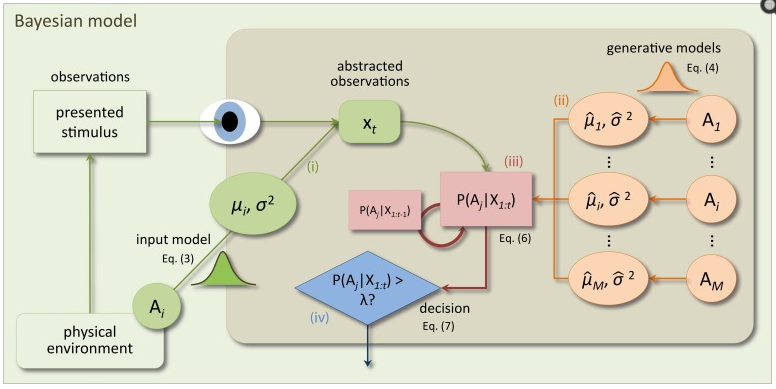
\includegraphics[width=1\textwidth]{figures/bayesian.PNG}}
	\caption{model bayesian}
	\label{bayesian}
	\end{figure}

Untuk kasus ini, proses input digunakan sebagai perkiraan masukan sensoris aktual yang ditunjukkan pada subjek. Gambar Gambar 11 menyajikan skematik model Bayesian dan keempat komponennya. Untuk setiap komponen, kami bertujuan untuk memilih formulasi yang paling sederhana agar sesuai dengan kesederhanaan matematika dari pDDM. Berikut ini kami rinci pilihan kita untuk keempat komponen ini.

\section {Mengisi model hirarkis}
Kelas HDDM menyusun DDM hirarkis yang ini nantinya sesuai dengan data RT dan pilihan subjek. 
Dengan tidak memberikan argumen tambahan selain data, HDDM membuat model yang sederhana dengan tidak memperhitungkan kondisi yang  berbeda. 
Untuk mempercepat konvergensi, titik awal diatur ke nilai a-posterior maksimum (MAP) dengan memanggil metode HDDM.find starting values yang menggunakan optimasi pendakian terhadap gradien. 
Metode HDDM.sample () kemudian melakukan inferensi Bayesian dengan menggambar sampel posterior menggunakan algoritma MCMC.

\begin{verbatim}

# memberi contoh objek model yang melampaui data kita

# ini akan menyesuaikan ddm hirarkis individu di sekitar kumpulan data

m = hddm.HDDM (data)

# temukan titik awal yang baik yang membantu konvergensi

m.find_starting_values ()

# mulai mengerjakan 2000 sampel dan membuang 20 dengan cara pembakaran

m.sample (2000, burn=20)

\end{verbatim}

\section Rational Model atau Classical Model
Model rasional adalah usaha pertama untuk mengetahui proses pengambilan keputusan. Hal ini dianggap oleh beberapa orang sebagai pendekatan klasik untuk memahami proses pengambilan keputusan. Model klasik memberikan berbagai langkah dalam proses pengambilan keputusan yang telah dibahas sebelumnya.

Fitur Model Klasik:
1. Masalahnya sudah jelas.
2. Tujuan sudah jelas.
3. Orang setuju dengan kriteria dan bobot.
4. Semua alternatif diketahui.
5. Semua konsekuensi bisa diantisipasi.
6. Keputusan membuat rasional.

\section Bounded Rationality Model or Administrative Man Model
Model Rationality Bounded didasarkan pada konsep yang dikembangkan oleh Herbert Simon. Model ini tidak menganggap rasionalitas individu dalam proses pengambilan keputusan.

Sebaliknya, ini mengasumsikan bahwa orang-orang, sementara mereka mungkin mencari solusi terbaik, biasanya menyelesaikan lebih sedikit, karena keputusan yang mereka hadapi biasanya menuntut informasi, waktu, kemampuan pemrosesan yang lebih besar daripada yang mereka miliki. Mereka puas dengan "rasionalitas terbatas atau rasionalitas terbatas dalam keputusan. Model ini didasarkan pada konsep dasar tertentu.

a. Sequential Attention to alternative solution
Biasanya kecenderungan orang untuk memeriksa kemungkinan solusi satu per satu daripada mengidentifikasi semua solusi yang mungkin dan berhenti mencari sekali solusi yang dapat diterima (walaupun tidak harus yang terbaik) ditemukan.

b. Heuristis:

Inilah asumsi yang memandu pencarian alternatif ke daerah-daerah yang memiliki probabilitas tinggi untuk menghasilkan kesuksesan.

c. Satisficing
Herbert Simon menyebut "kepuasan" ini yang memilih tindakan yang memuaskan atau "cukup baik" dalam situasi seperti ini. Kecenderungan bagi pengambil keputusan untuk menerima alternatif pertama yang memenuhi persyaratan minimal yang dapat diterima daripada mendorong mereka lebih jauh untuk sebuah alternatif yang menghasilkan hasil terbaik.
